\documentclass[notheorems, handout, 10pt]{beamer}

\usetheme[numbers,totalnumbers,compress, nologo]{Statmod}
\usefonttheme[onlymath]{serif}
\setbeamertemplate{navigation symbols}{}

\mode<handout> {
	\usepackage{pgfpages}
	%\setbeameroption{show notes}
	%\pgfpagesuselayout{2 on 1}[a4paper, border shrink=5mm]
	\setbeamercolor{note page}{bg=white}
	\setbeamercolor{note title}{bg=gray!10}
	\setbeamercolor{note date}{fg=gray!10}
}

\usepackage[utf8x]{inputenc}
\usepackage[T1,T2A]{fontenc}
\usepackage[russian]{babel}

\usepackage{amsmath,amsthm,amssymb}
\usepackage{mathtext}
\usepackage{graphicx}

\title[Embeddings]{Embeddings}
\author[Самарин И.А.]{Самарин Игорь, группа 23.М03-мм}
\institute{Санкт-Петербургский государственный университет\\Кафедра статистического моделирования}
\date{\vspace{3cm}\\Санкт-Петербург\\2024 г.}

\subject{Talks}

\setbeamertemplate{caption}[numbered]

\setbeamercolor{bluetext_color}{fg=blue}
\newcommand{\bluetext}[1]{{\usebeamercolor[fg]{bluetext_color}#1}}

\begin{document}
	
	\listoftables

	\begin{frame}[plain]
		
		\titlepage
		
		\note{ 
			
		}
		
	\end{frame}
	
	\begin{frame}{Введение}
		
		\textsl{Обработка естественного языка} "--- это область, посвященная анализу текстов, написанных на естественных (человеческих) языках. 
		
		\vspace{0.2cm}
		
		Различают четыре режима работы с текстовыми данными:
		\begin{itemize}
			\item \textbf{Many-to-one}: на входе последовательность объектов, на выходе один объект;
			\item \textbf{One-to-many}: на входе один объект, на выходе последовательность объектов;
			\item \textbf{Many-to-many}: на входе и выходе последовательности нефиксированной длины;
			\item \textbf{Синхронизированный many-to-many}: на входе и выходе последовательности фиксированной длины, токены входной последовательности явно сопоставлены токенам выходной.
		\end{itemize}
		
		Перед рассмотрением архитектур, необходимо разобраться с базовыми понятиями о нейронных сетях.
		
		\note{
			
		}
		
	\end{frame}
	
	\begin{frame}{Нейронная сеть. Определение}
		
		\textsl{Искусственная нейронная сеть} "--- это сложная дифференцируемая функция, задающая отображение из исходного пространства в пространство ответов, все параметры которой могут настраиваться одновременно и взаимосвязанно.
		
		\vspace{0.2cm}
		
		Сложную функцию удобно представлять в виде суперпозиции простых. Простейшие разновидности:
		\begin{itemize}
			\item \textbf{Линейный слой}: линейное преобразование над входящими данными. Обучаемые параметры "--- матрица $W$ и вектор $b$ такие, что $x \mapsto xW + b$, где $(W \in \mathbb{R}^{d\times k}, x \in \mathbb{R}^{d}, b \in \mathbb{R}^{k})$;
			\item \textbf{Функция активации}: нелинейное преобразование, поэлементно применяющееся к пришедшим на вход данным.
		\end{itemize}
		
		Таким образом, нейронную сеть можно представить в виде вычислительного графа, где промежуточным вершинам соотствуют преобразования.
		
		\note{
			
		}
	
	\end{frame}
	
	\begin{frame}{Нейронная сеть}
		
		\begin{figure}[H]
			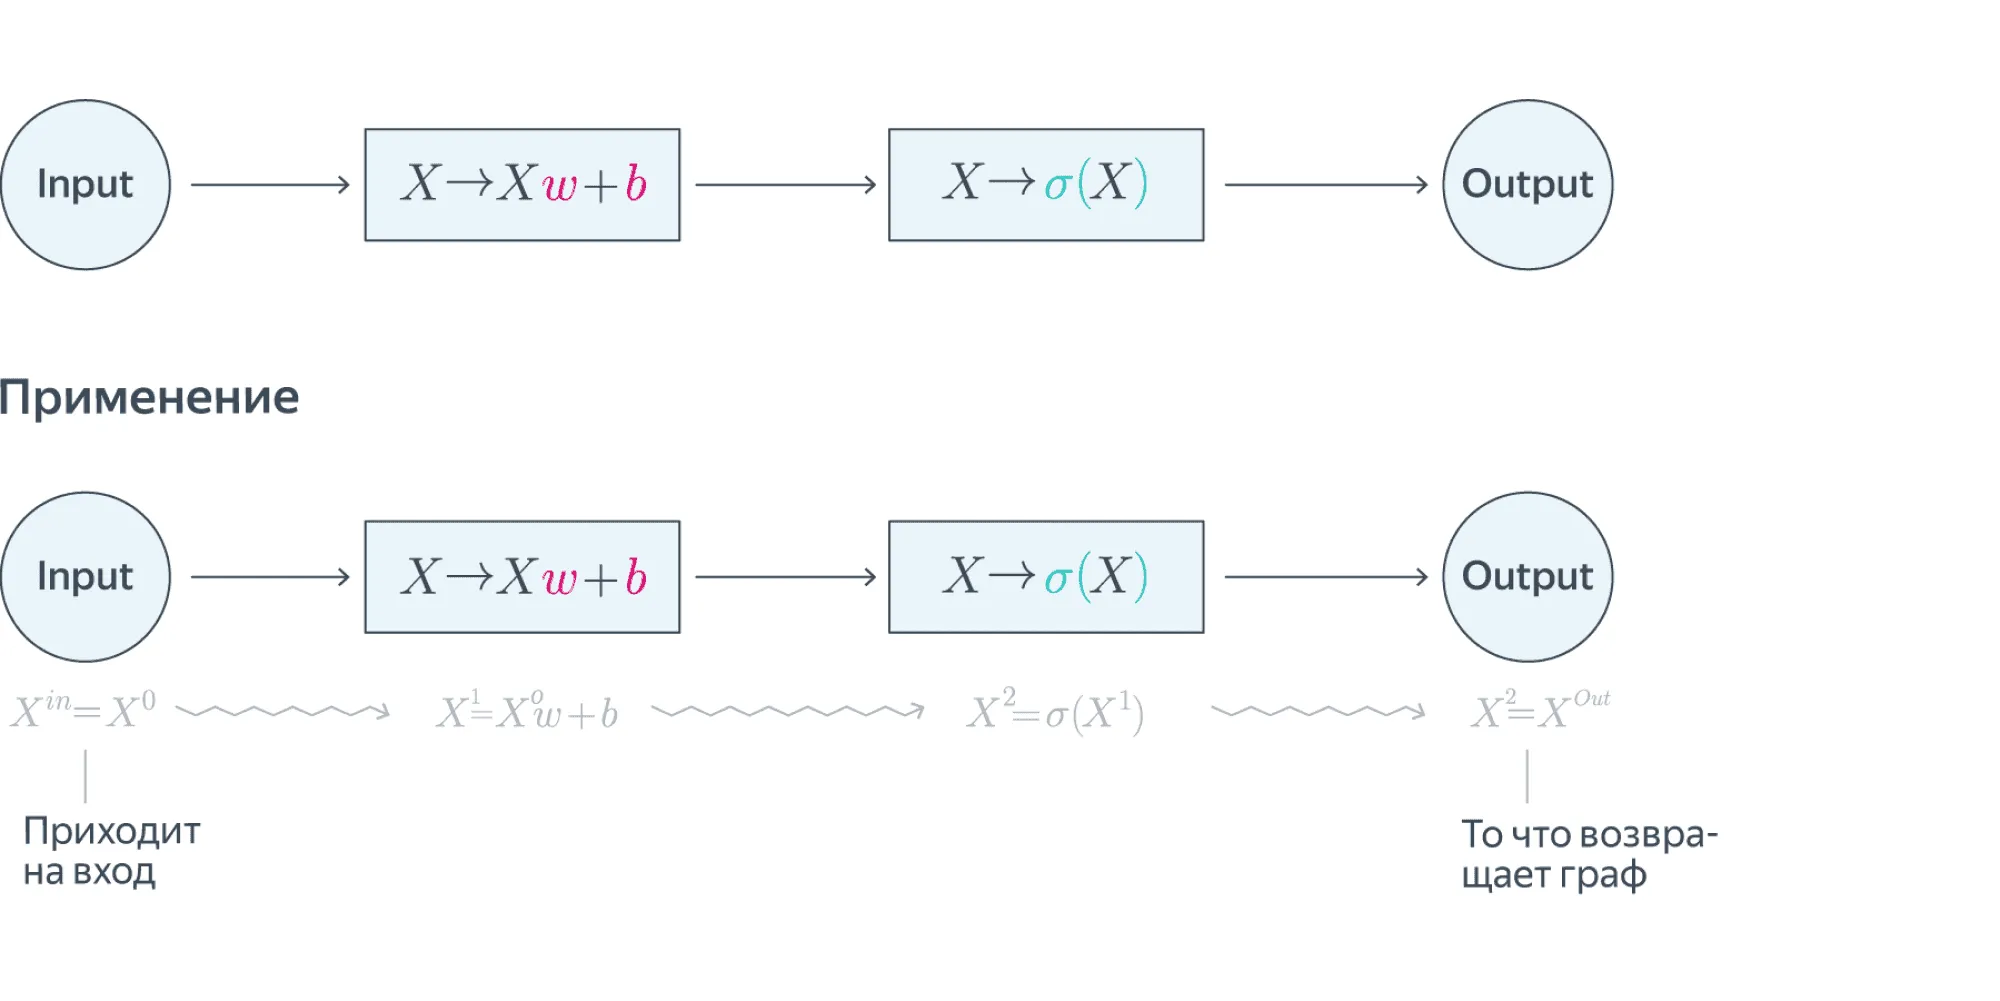
\includegraphics[width=1\linewidth]{images/1}
		\end{figure}
		
		\note{
			
		}
		
	\end{frame}
	
	\begin{frame}{Нейронная сеть. Forward propagation}
		
		Применение нейронной сети к данным (вычисление выхода по заданному входу) назвается \textsl{прямым проходом} (forward propagation).
		
		\begin{figure}[H]
			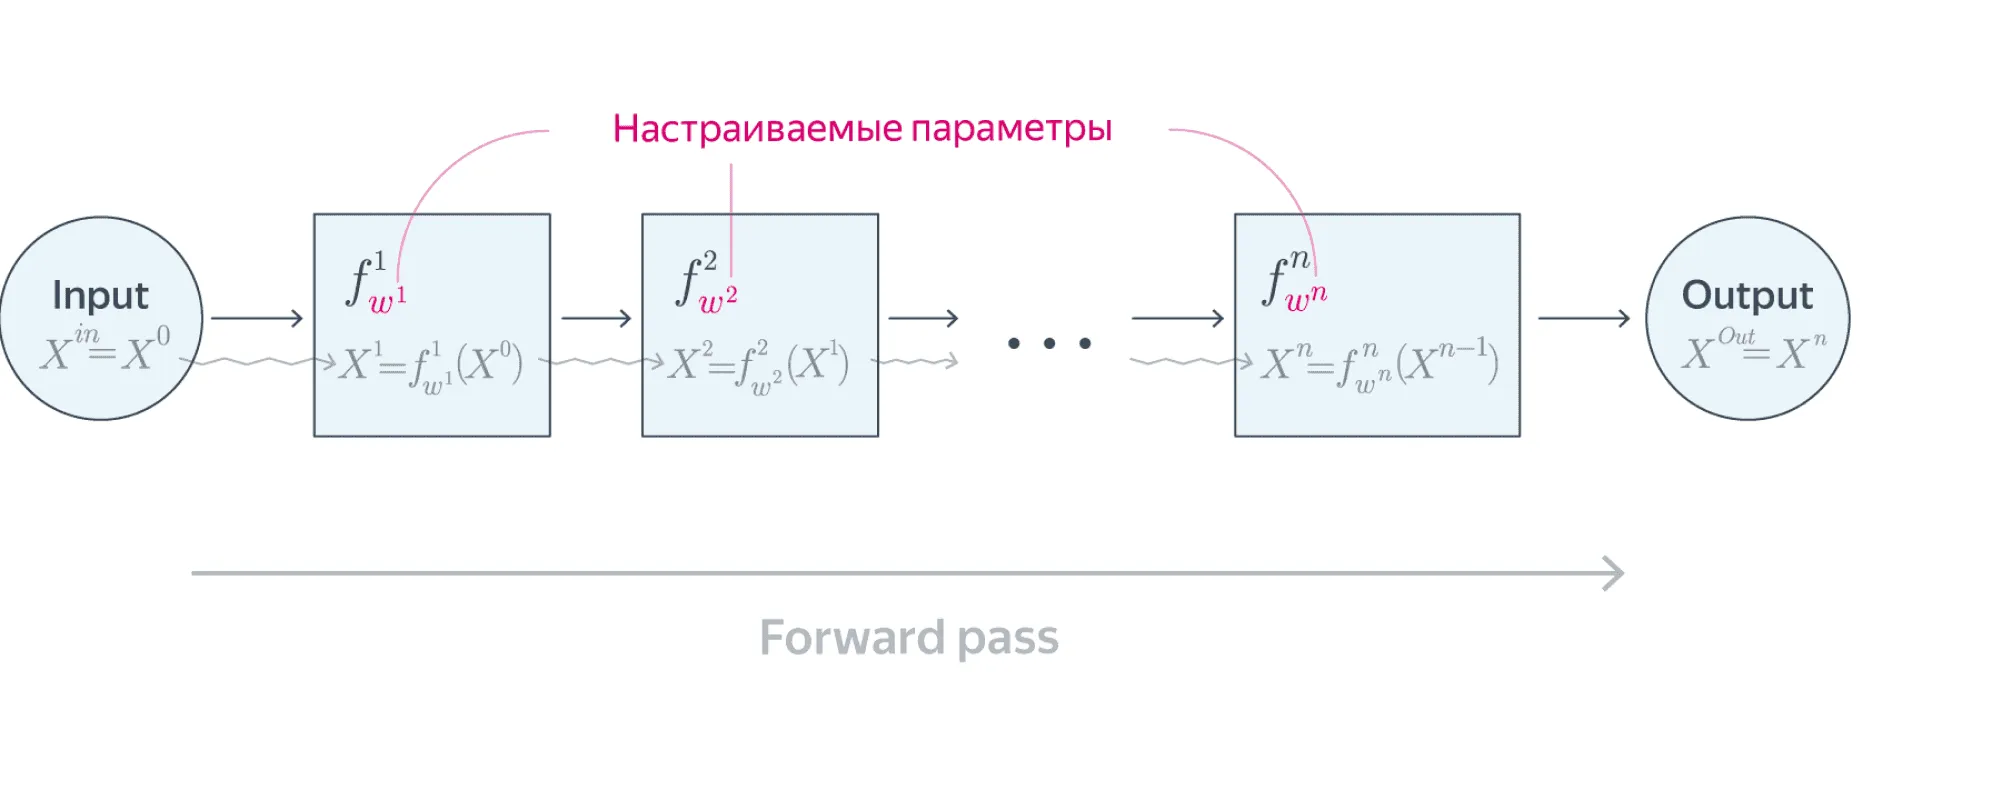
\includegraphics[width=1\linewidth]{images/2}
		\end{figure}
		
		На этом этапе происходит преобразование исходного представления данных в целевое.
		
		\note{
			
		}
		
	\end{frame}
	
	\begin{frame}{Нейронная сеть. Backward propagation}
		
		При \textsl{обратном проходе} (backward propagation), информация (обычно об ошибке предсказания) движется от финального представления к исходному через все преобразования.
		
		\begin{figure}[H]
			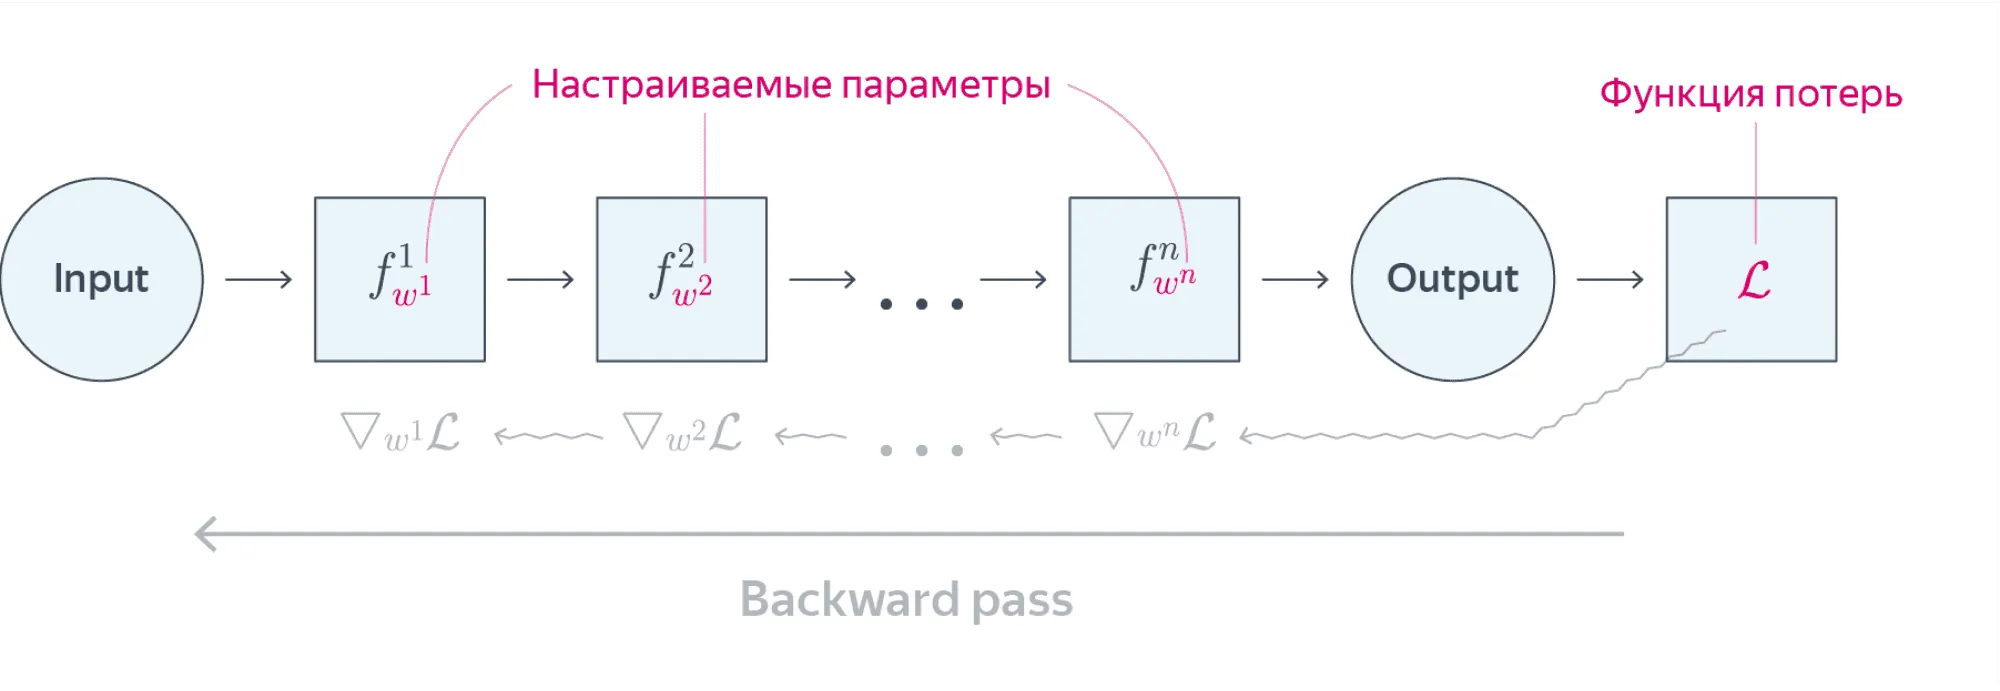
\includegraphics[width=1\linewidth]{images/3}
		\end{figure}
		
		\note{
			
		}
		
	\end{frame}
	
	\begin{frame}{Нейронная сеть. Backward propagation в одномерном случае}
		
		Пусть $\omega_0$ "--- переменная, по которой хотим продифференцировать сложную функцию вида: $$f(\omega_0)=g_m(g_{m-1}(\dots g_1(\omega_0)\dots)),$$ где все $g_i$ скалярные.
		
		\vspace{0.2cm}
		
		Тогда производная имеет вид: $$\resizebox{0.9\textwidth}{0.9\height}{$f'(\omega_0)=g'_m(g_{m-1}(\dots g_1(\omega_0)\dots))\cdot g'_{m-1}(g_{m-2}(\dots g_1(\omega_0)\dots))\cdot\dots\cdot g'_1(\omega_0),$}$$ где $g_1(\omega_0), g_2(g_1(\omega_0)), \dots, g_{m-1}(\dots g_1(\omega_0)\dots)$ известны.
		
		\vspace{0.2cm}

		Как правило, на практике пользуются матричными вычислениями.
		
		\note{
			
		}
		
	\end{frame}
	
	\begin{frame}{Word Embeddings. Статистические подходы}
		
		Прежде чем подавать текстовые данные на вход нейросети, их необходимо векторизировать. 
		
		\vspace{0.2cm}
		
		К векторизации текстов есть два базовых подхода:

		\begin{itemize}
			\item Векторизовать текст целиком, превращая его в один вектор;
			\item Векторизовать отдельные структурные единицы, превращая текст в последовательность векторов.
		\end{itemize}
		
		Самый простой вариант "--- Bag-of-Words. Текст представляется в виде вектора частот встречаемости каждого токена.
		
		\vspace{0.2cm}
		
		Чуть более сложный "--- TF-IDF. Представление текста $d$ состоит из произведений $TF(t, d)\cdot IDF(t, D)$ по всем токенам $t$ из коллекции $D$, где $TF(t, d)=\frac{n_t}{\sum_k^{}n_k}$, а $IDF(t, D)=\log\frac{|D|}{|\{d_i\in D | t\in d_i\}|}$.
		
		\note{
			
		}
		
	\end{frame}
	
	\begin{frame}{Word Embeddings. Word2vec}
		
		Word2vec "--- способ построения сжатого пространства векторов слов, использующий нейронные сети. 
		
		\vspace{0.2cm}
		
		Для обучения авторы предлагают две стратегии:
		\begin{itemize}
			\item \textbf{CBOW}: модель учится предсказывать данное (центральное) слово по контексту;
			\item \textbf{Skip-gram}: модель учится по данному слову предсказывать контекст.
		\end{itemize}
		
		\vspace{0.2cm}
		
		Нейросеть учит векторы слов так, чтобы скалярное произведение между векторами двух слов, которые часто используются в контексте, были как можно больше.
		
		\note{
			
		}
		
	\end{frame}
	
	\begin{frame}{Word Embeddings. Word2vec}
		
		\begin{figure}[H]
			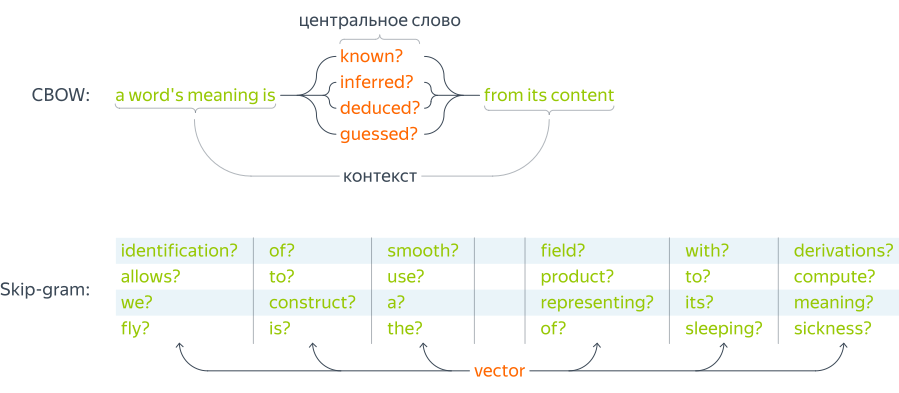
\includegraphics[width=1\linewidth]{images/4}
		\end{figure}
		
		\note{
			
		}
		
	\end{frame}
	
	\begin{frame}{Word Embeddings. Word2vec. CBOW}
		
		В модели CBOW вычисляются $logits_u=<\sum_{w\in context} v_w, v_u>$, после чего "--- вероятности всевозможных слов $u$ быть центральными для контекста как $softmax(logits)$.
		
		\begin{figure}[H]
			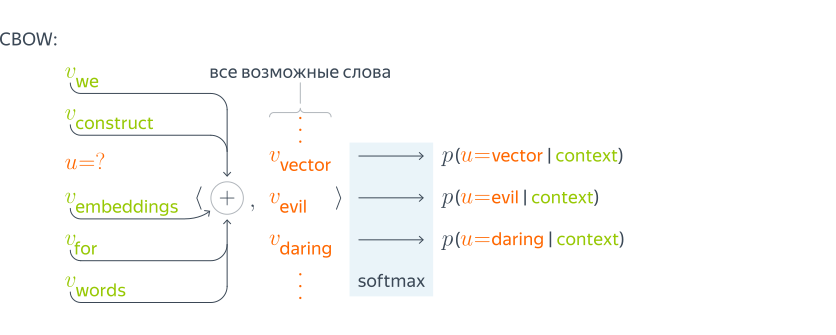
\includegraphics[width=0.7\linewidth]{images/cbow}
		\end{figure}
		
		Модель учится на кросс-энтропию полученного распределения с истинным распределением центральных слов.
		
		\note{
			
		}
		
	\end{frame}
	
	\begin{frame}{Word Embeddings. Word2vec. SkipGram}
		
		В модели Skip-gram по центральному слову $u$ для каждой позиции контекста предсказывается распределение вероятностей. 
		
		\begin{figure}[H]
			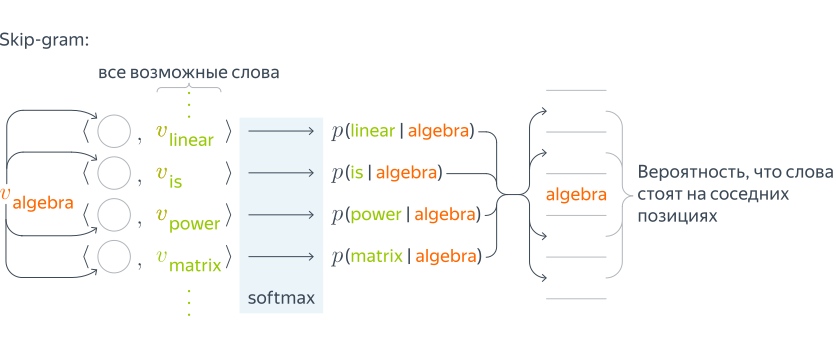
\includegraphics[width=0.7\linewidth]{images/skipgram}
		\end{figure}
		
		Функция потерь: сумма кросс-энтропий распределений слов контекста с их истинными распределениями.
			
		\note{
	
		}
		
	\end{frame}
	
	\begin{frame}{Word Embeddings. Word2vec. Особенности}
		
		Векторы содержат "смысл" слов. Два вектора можно сравнивать при помощи косинусного расстояния.
		
		\begin{figure}[H]
			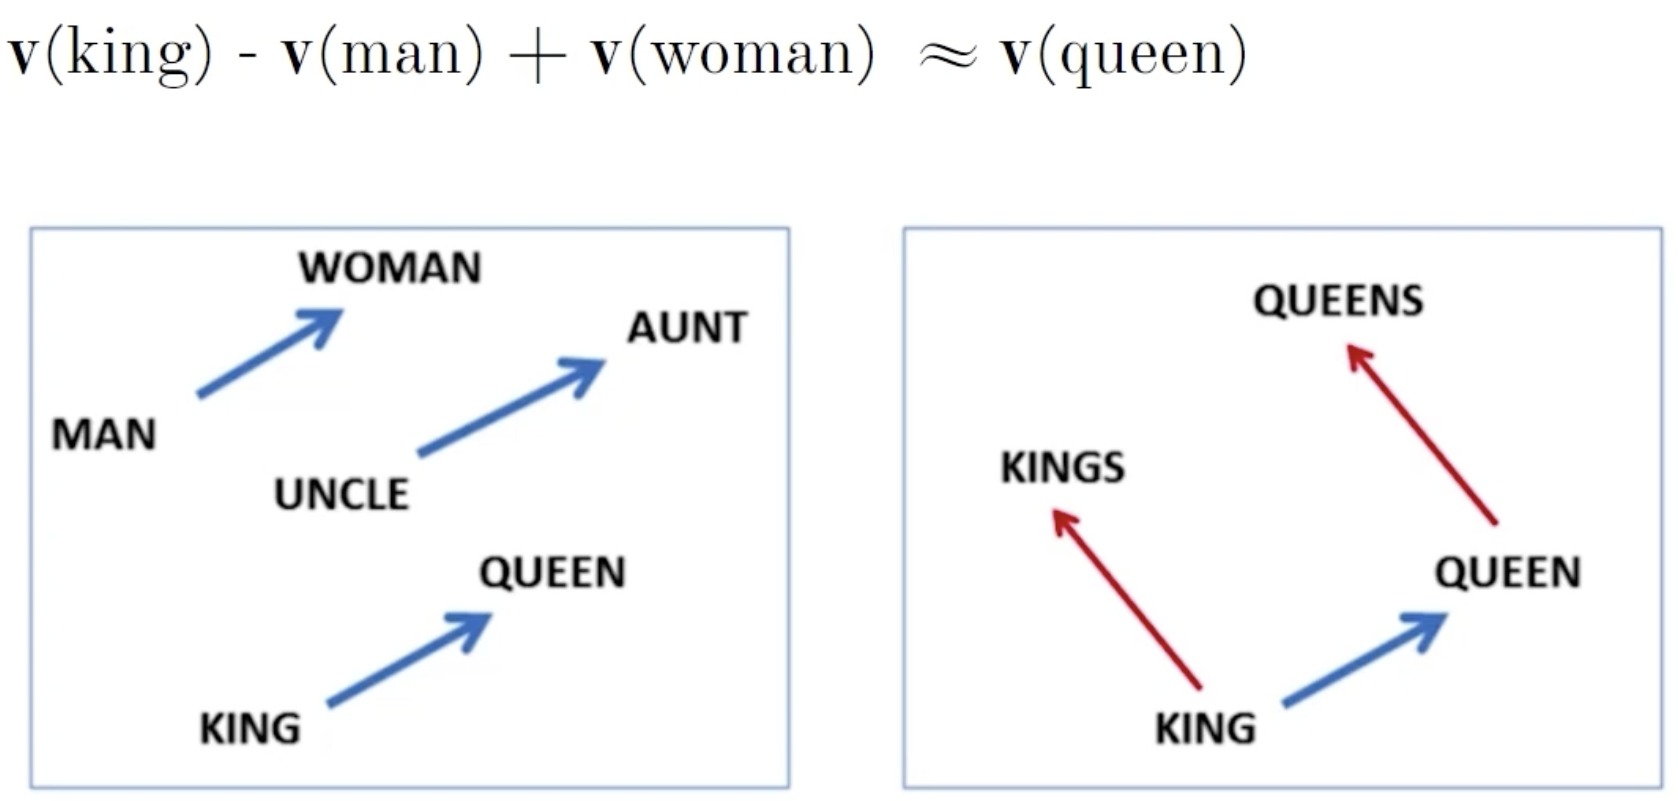
\includegraphics[width=0.7\linewidth]{images/king}
		\end{figure}
				
		\note{
			
		}
		
	\end{frame}
	
	\begin{frame}{Word Embeddings. Word2vec. Преимущества и недостатки}
		
		Преимущества:
		\begin{itemize}
			\item Векторы отражают смысл слов;
			\item Размерность векторов не зависит от размера словаря;
			\item При добавлении документов векторы можно дообучить.
		\end{itemize}
		
		\vspace{0.2cm}
		
		Недостатки:
		\begin{itemize}
			\item Фиксированный размер словаря;
			\item Для редких слов эмбеддинги получаются неоптимальными;
			\item Слова имеющие один корень, обрабатываются по-разному.
		\end{itemize}
		
		\note{
			
		}
		
	\end{frame}
	
	\begin{frame}{Word Embeddings. FastText}
		
		Библиотека FastText является технической модификацией Word2Vec.
		
		\vspace{0.2cm}
		
		Модель sub-word: разделим слова на буквенные $n$-граммы, тогда вектор слова будет сумма векторов его $n$-грамм.
		
		\vspace{0.2cm}
		
		Преимущества:
		\begin{itemize}
			\item Можно получать более адекватные эмбеддинги для редких и неизвестных слов;
		\end{itemize}
		
		\vspace{0.2cm}
		
		Недостатки:
		\begin{itemize}
			\item $n$-грамм может быть очень много;
			\item Требуется больше вычислительных ресурсов.
		\end{itemize}
		
		\note{
			
		}
		
	\end{frame}
	
\end{document}